% !TEX root = ./Basilisk-Integrators20170724.tex


\begin{figure}[htb]
	\centerline{
	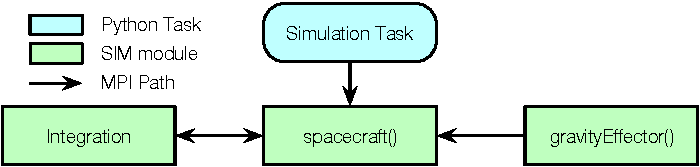
\includegraphics[]{Figures/integratorDiagram}
	}
	\caption{Illustration of the Integrator Diagram}
	\label{fig:intDiag}
\end{figure}


\section{Model Description}

\subsection{Overview}
The Basilisk integration capability is implemented in a modular manner such that different integrators can be assigned to the equations of motion that must be solved.  Figure~\ref{fig:intDiag} illustrates how the integrator functions relative to a dynamical systems model, here the {\tt spacecraft()} object.  The ODE's are provided by a sub-class of {\tt DynamicObject} which must be able to respond to the {\tt equationsOfMotion()} method.  Integration of the state vector forward one time step is then handled by the {\tt integrate} method of the integrator class.  By default the {\tt DynamicObject} is integrated using a fixed time step 4th order Runge-Kutta method.

Assume the dynamical system is given by
\begin{equation}
	\dot{\bm x} = \bm f(t, \bm x)
\end{equation}
The initial conditions are specified through $\bm x_{0} = \bm x(t_{0})$.  In integration time step is given through $h$.  

\subsection{Implemented Integrators}

\subsubsection{4th Order Runge Kutta - Default Integrator}
A standard fixed time step 4th order Runge Kutta integrator is enabled by default.  The 4 $k_{i}$ values are defined as
\begin{align}
	\bm k_{1} &= \bm f\left(t_{n}, \bm x_{n}\right) \\
	\bm k_{2} &= \bm f\left(t_{n} + \frac{h}{2}, \bm x_{n} + \frac{h}{2} \bm k_{1}\right) \\
	\bm k_{3} &= \bm f\left(t_{n} + \frac{h}{2}, \bm x_{n} + \frac{h}{2} \bm k_{2}\right) \\
	\bm k_{4} &= \bm f\left(t_{n} + h, \bm x_{n} + h \bm k_{3}\right) 
\end{align}
The state at the next integration time $t_{n+1} = t_{n} + h$ is
\begin{equation}
	\bm x_{n+1} = \bm x_{n} + \frac{h}{6} \left(
		\bm k_{1} + 2 \bm k_{2} + 2 \bm k_{3} + \bm k_{4}
	\right)
\end{equation}


\subsubsection{2nd Order Runge Kutta (Heun's Method)}
A 2nd order Runge-Kutta method is implemented through Heun's method.\footnote{\url{http://goo.gl/SWdyBZ}} The 2 $k_{i}$ values are defined as
\begin{align}
	\bm k_{1} &= \bm f(t_{n}, \bm x_{n}) \\
	\bm k_{2} &= \bm f(t_{n} + h, \bm x_{n} + h \bm k_{1}) 
\end{align}
The state at the next integration time $t_{n+1} = t_{n} + h$ is
\begin{equation}
	\bm x_{n+1} = \bm x_{n} + \frac{h}{2} \left(
		\bm k_{1} +  \bm k_{2}
	\right)
\end{equation}


\subsubsection{1st Order Runge Kutta (Euler's Method)}
A first order Runge-Kutta method is implemented through Euler's method. The one $k_{1}$ value is defined as
\begin{align}
	\bm k_{1} &= \bm f(t_{n}, \bm x_{n}) 
\end{align}
The state at the next integration time $t_{n+1} = t_{n} + h$ is
\begin{equation}
	\bm x_{n+1} = \bm x_{n} + h
		\bm k_{1}
\end{equation}

\subsubsection{4th Order Runge Kutta Fehlberg Variable Time Step}
A fourth order Runge-Kutta-Fehlberg is implemented. It propagates the state using a fourth order integration method, while comparing the resulting truncation error with a fifth order integration method. The $k_i$ values are defined as
\begin{align}
	\bm k_1 &= \bm f\left(t_{n}, \bm x_{n}\right) \label{eq:k1_RKF45}\\
	\bm k_2 &= \bm f\left(t_{n} + \frac{h}{4}, \bm x_{n} + \frac{h}{4} \bm k_1\right) \\
	\bm k_3 &= \bm f\left(t_{n} + \frac{3h}{8}, \bm x_{n} + \frac{3h}{32} \bm k_1 + \frac{9h}{32} \bm k_2\right) \\
	\bm k_4 &= \bm f\left(t_{n} + \frac{12h}{13}, \bm x_{n} + \frac{1932h}{2197} \bm k_1 - \frac{7200h}{2197} \bm k_2 + \frac{7296h}{2197} \bm k_3\right) \\
	\bm k_5 &= \bm f\left(t_{n} + h, \bm x_{n} + \frac{439h}{216} \bm k_1 - 8h \bm k_2 + \frac{3680h}{513} \bm k_3 - \frac{8450h}{4104} \bm k_4\right) \\
	\bm k_6 &= \bm f\left(t_{n} + \frac{h}{2}, \bm x_{n} - \frac{8h}{27} \bm k_1 + 2h \bm k_2 - \frac{3544h}{2565} \bm k_3 + \frac{1859h}{4104} \bm k_4 - \frac{11h}{40} \bm k_5\right) \label{eq:k6_RKF45}
\end{align}
The state at the next integration time $t_{n+1} = t_{n} + h$ is
\begin{equation}
	\bm x_{n+1} = \bm x_{n} + h \left(
		\frac{25}{216} \bm k_{1} + \frac{1408}{2565} \bm k_{3} + \frac{2197}{4104} \bm k_{4} - \frac{1}{5} \bm k_{5} \label{eq:PropagateState_RKF45}
	\right)
\end{equation}
The estimate for the relative truncation error is
\begin{equation}
	\bm \delta = h\frac{\left\|
		\frac{1}{360} \bm k_{1} - \frac{128}{4275} \bm k_{3} - \frac{2197}{75240} \bm k_{4} - \frac{1}{50} \bm k_{5} + \frac{2}{55} \bm k_{6} \label{eq:Error_RKF45}
	\right\|}{\|\bm x_n\|}
\end{equation}
The updated time step is calculated through the following equation
\begin{equation}
	h_{\text{new}}=0.9h\left(\frac{\bm \epsilon}{\bm \delta}\right)^{1/5}, \label{eq:h_RKF45}
\end{equation}
where $\bm \epsilon$ corresponds to the relative tolerance and its default value is $10^{-4}$. If the norm of the state is smaller than the absolute tolerance (default value of $10^{-8}$), the relative error is calculated with respect to that absolute tolerance instead of the true vector norm. The time step is scaled by $0.9$ for robustness, so that the integrator will not use values that barely pass through the relative tolerance.\\
The algorithm for the variable time step integrator works as follows:
\begin{enumerate}
	\item For every state vector, compute the $\bm k_i$ integration weights through equations \ref{eq:k1_RKF45}-\ref{eq:k6_RKF45}.
	\item Propagate the state to the next time step using those weights using equation \ref{eq:PropagateState_RKF45}.
	\item For every state, calculate the relative truncation error (\ref{eq:Error_RKF45}) and store the largest value of all the state errors.
	\item Compute the new time step through \ref{eq:h_RKF45}.
	\item If the relative truncation error $\bm \delta$ is larger than the relative tolerance $\bm \epsilon$, repeat steps 1-4 with the new time step until it does.
	\item Update the integration time with the time step used during integration: $t_{n+1} = t_n + h$.
	\item Update the integration time step with the new time step: $h = h_{\text{new}}$.
	\item Check if the new time step would overpass the final integration time. If it does, change it so that $h = t_f - t_{n+1}$.
	\item Go back to step 1 until the final integration time has been reached.
\end{enumerate}

\subsubsection{7th Order Runge Kutta Fehlberg Variable Time Step}
A seventh order Runge-Kutta-Fehlberg is implemented. It propagates the state using a seventh order integration method, while comparing the resulting truncation error with an eighth order integration method. The $k_i$ values are defined in a general way as
\begin{align}
	\bm k_1 &= \bm f\left(t_{n} + \bm\alpha_1 h, \bm x_{n} \right)\\
	\bm k_i &= \bm f\left(t_{n} + \bm\alpha_i h, \bm x_{n} + h \sum_{j=1}^{i-1}\bm\beta_{ij} \bm k_j\right), \quad i=2,...,13
\end{align}
where the $\bm\alpha$ and $\bm\beta$ matrices are defines as
\setcounter{MaxMatrixCols}{15}
\begin{align}
	\bm \alpha = \begin{bmatrix}
		0\\[6pt]
		\frac{2}{27}\\[6pt]
		\frac{1}{9}\\[6pt]
		\frac{1}{6}\\[6pt]
		\frac{5}{12}\\[6pt]
		\frac{1}{2}\\[6pt]
		\frac{5}{6}\\[6pt]
		\frac{1}{6}\\[6pt]
		\frac{2}{3}\\[6pt]
		\frac{1}{3}\\[6pt]
		1\\[6pt]
		0\\[6pt]
		1
	\end{bmatrix} \quad \bm \beta=\begin{bmatrix}
		& & & & & & & & & & & & \\[6pt]
		\frac{2}{27} & & & & & & & & & & & \\[6pt]
		\frac{1}{36} & \frac{1}{12} & & & & & & & & & & \\[6pt]
		\frac{1}{24} & 0 & \frac{1}{8} & & & & & & & & & \\[6pt]
		\frac{5}{12} & 0 & -\frac{25}{16} & -\frac{25}{16} & & & & & & & & \\[6pt]
		\frac{1}{20} & 0 & 0 & \frac{1}{4} & \frac{1}{5} & & & & & & & \\[6pt]
		-\frac{25}{108} & 0 & 0 & \frac{125}{108} & -\frac{65}{27} & \frac{125}{54} & & & & & & \\[6pt]
		\frac{31}{300} & 0 & 0 & 0 & \frac{61}{225} & -\frac{2}{9} & \frac{13}{900} & & & & & \\[6pt]
		2 & 0 & 0 & -\frac{53}{6} & \frac{704}{45} & -\frac{107}{9} & \frac{67}{90} & 3 & & & & \\[6pt]
		-\frac{91}{108} & 0 & 0 & \frac{23}{108} & -\frac{976}{135} & \frac{311}{54} & -\frac{19}{60} & \frac{17}{6} & -\frac{1}{12} & & & \\[6pt]
		\frac{2383}{4100} & 0 & 0 & -\frac{341}{164} & \frac{4496}{1025} & -\frac{301}{82} & \frac{2133}{4100} & \frac{45}{82} & \frac{45}{164} & \frac{18}{41} & & \\[6pt]
		\frac{3}{205} & 0 & 0 & 0 & 0 & -\frac{6}{41} & -\frac{3}{205} & -\frac{3}{41} & \frac{3}{41} & \frac{6}{41} & 0 & \\[6pt]
		-\frac{1777}{4100} & 0 & 0 & -\frac{341}{164} & \frac{4496}{1025} & -\frac{289}{82} & \frac{2193}{4100} & \frac{51}{82} & \frac{33}{164} & \frac{12}{41} & 0 & 1
	\end{bmatrix}
\end{align}
The state at the next integration time $t_{n+1} = t_{n} + h$ is
\begin{equation}
	\bm x_{n+1} = \bm x_{n} + h \sum_{i=1}^{13}\text{CH}(i)\bm k_i
\end{equation}
and the truncation error is
\begin{align}
	\bm \delta = h\frac{\left\|
		\sum_{i=1}^{13}\text{CT}(i)\bm k_i \label{eq:Error_RKF78}
	\right\|}{\|\bm x_n\|}
\end{align}
The CH and CT matrices are given by
\begin{align}
	\text{CH} = \begin{bmatrix}
		0\\[6pt]
		0\\[6pt]
		0\\[6pt]
		0\\[6pt]
		0\\[6pt]
		\frac{34}{105}\\[6pt]
		\frac{9}{35}\\[6pt]
		\frac{9}{35}\\[6pt]
		\frac{9}{280}\\[6pt]
		\frac{9}{280}\\[6pt]
		0\\[6pt]
		\frac{41}{840}\\[6pt]
		\frac{41}{840}
	\end{bmatrix} \qquad \text{CT} = \begin{bmatrix}
		-\frac{41}{840}\\[6pt]
		0\\[6pt]
		0\\[6pt]
		0\\[6pt]
		0\\[6pt]
		0\\[6pt]
		0\\[6pt]
		0\\[6pt]
		0\\[6pt]
		0\\[6pt]
		-\frac{41}{840}\\[6pt]
		\frac{41}{840}\\[6pt]
		\frac{41}{840}
	\end{bmatrix}
\end{align}
The algorithm used to update the time step is the same as the one described for the 4th order variable time step integrator.
